\chapter{Apprendimento e Risultati}
\label{cap4}
\setcounter{figure}{0}

La metodologia proposta nei precedenti capitoli verrà sistematicamente valutata in questo capitolo. Mostreremo i risultati ottenuti utilizzando le features individuate nel secondo capitolo, con i dati raccolti come esposto nel capitolo precedente. In Fig 2 riporto un diagramma di flusso redatto da Sebastian Raschka, il quale dà un'ottima visione globale della la pipeline di processi affrontati nell'apprendimento supervisionato e quindi quelli di questo capitolo. Come metriche per misurare la bontà del modello di classificazione useremo, l'Accuracy (ACC), la F-measure (F1), e la Area Under Curve (AUC) della funzione Receiver Operating Characteristic (ROC), brevemente illustrate qui sotto.
Uno strumento tipico per valutare la performance è la così conosciuta “matrice di confusione”, una matrice quadrata che consiste in colonne e righe che descrivono il numero di istanze come il rapporto tra “classe attuale” e “classe predetta”. Una semplice matrice di confusione per il classico problema di classificazione di “spam vs. ham”, un classificatore che individua tra le email ricevute quelle che sono da considerare posta indesiderata, potrebbe essere quella riporta in Fig1. \newline L'accuratezza è definita come la frazione della classificazioni corrette su il numero totale di samples. È calcolata come:


\begin{figure}[bp!]
\centering
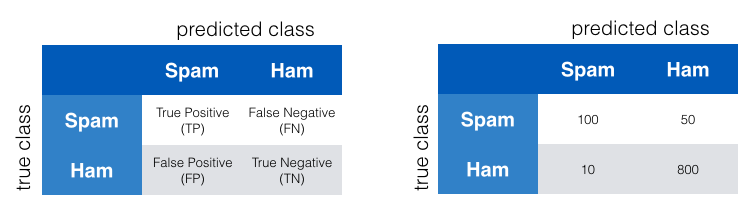
\includegraphics[width=130mm]{chapters/plots/confusion_matrix.png}
\caption{Matrice di confusione Spam vs Ham \label{overflow}}
\end{figure}

\begin{gather*}
	Accuracy = \frac{TP + TN}{TP + FP + TN + FN }
\end{gather*}

dove TP= True Positive, TN= True Negative, ovvero le istanze classificate correttamente, FP = False Positive, il numero di istanze classificate erroneamente positive, e FN = False Negative, il numero di istanze classificate erroneamente negative. Altri indicatori per le performance di un classificatore sono la Sensibilità o Recall e la Precision. Che si calcolano in questo modo:

\begin{gather*}
	Recall = \frac{TP}{TP + FN}
\end{gather*}

\begin{gather*}
	Precision = \frac{TP}{TP + FP}
\end{gather*}

La F-measure prende in considerazione sia la Precision che la Recall. Questa può essere interpretata come la media armonica pesata della Precision e la Recall. Spesso viene  utilizzata la F1-measure o \textit{balanced F-score} (F1 score), questa è la media armonica pesata con pesi unitari e si ottiene calcolando:

\begin{gather*}
	F1 = 2 \cdot \frac{TP \cdot FP}{TP + FP}
\end{gather*}


\begin{figure}[bp!]
\centering
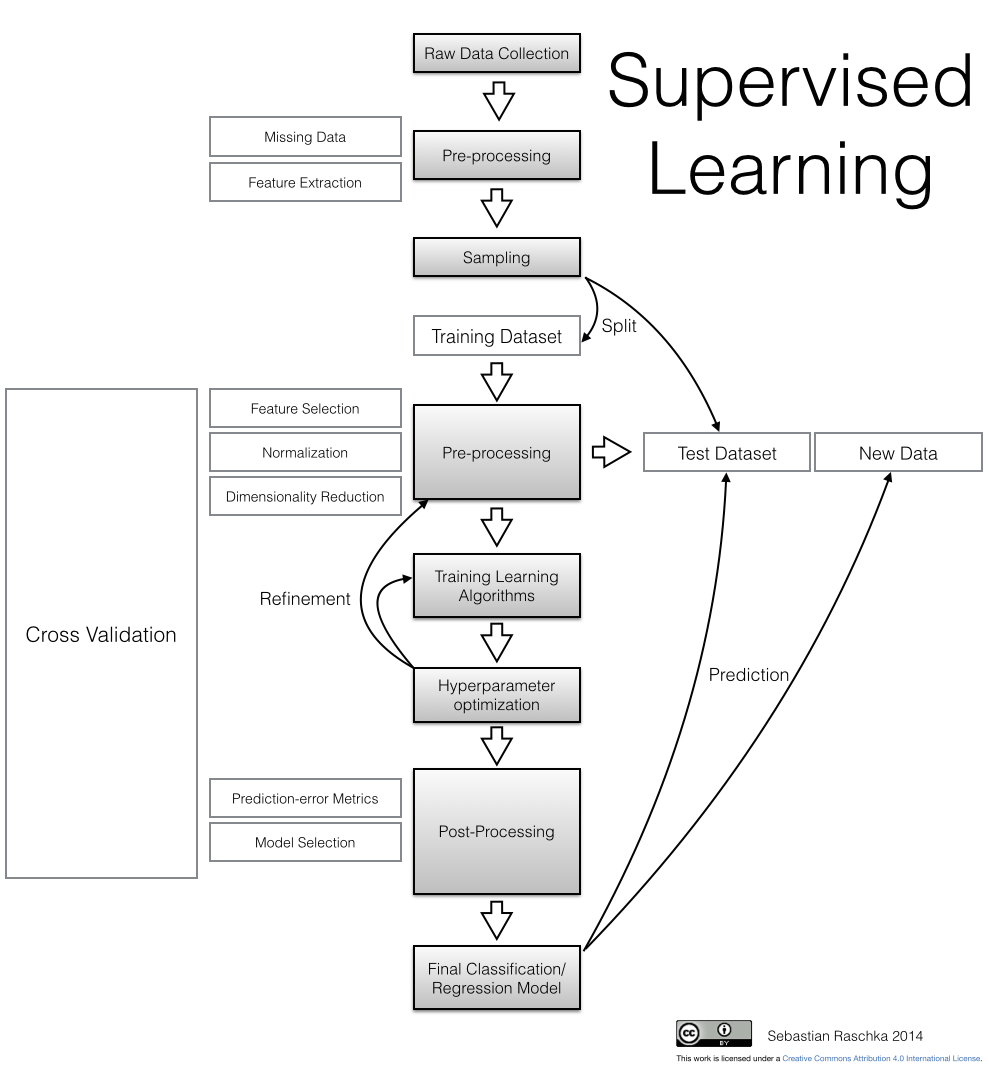
\includegraphics[width=130mm]{chapters/process_pipeline/supervised_learning_flowchart.png}
\caption{Supervised learning flowchart \label{overflow}}
\end{figure}

\section{Preprocessamento dei dati}
Per ogni profilo \textit{P} con un insieme di username \textit{U}, vogliamo creare una tupla:
\begin{gather*}
	(candidate, priors)
\end{gather*}
dove \textit{candidate} vale \textit{u} e \textit{priors}  vale \textit{u} $\setminus$ \textit{U}, per ogni usernames \textit{u} in \textit{U}.
\newline
Prima di estrarre le features dai samples del nostro dataset, dobbiamo preprocessare i dati acquisiti in modo da non avere sample con dati mancanti. Applicando le seguenti politiche:

\begin{itemize}
	\item l(\textit{candidate}) \textless 1 $\Rightarrow$ sample eliminato
	\item l(\textit{prior}) \textless 1 $\Rightarrow$ prior rimosso dalla lista di priors
	\item l(\textit{priors}) \textless 1 $\Rightarrow$ sample eliminato
\end{itemize}

dove \textit{l} è una funzione che ritorna la lunghezza di una stringa di caratteri o la cardinalità di un insieme di stringhe, otteniamo un dataset pulito che permetterà di evitare errori nella fase di estrazione delle features.\newline
I dati ottenuti rappresenteranno l'insieme dei nostri samples che verranno etichettati di classe positiva, ovvero samples di cui si riconosce l'attribuzione di ogni usernames verso un individuo \textit{I}. Un classificatore binario ha peró bisogno anche di samples etichettati con una seconda classe. Nel nostro caso siamo interessati a separare usernames associati a uno stesso individuo da quelli che non lo sono. Dovremmo quindi elaborare a partire dal nostro dataset un insieme di samples che verrano etichettati come esempi negativi, ovvero samples che non godono della proprietà elencata prima per i samples positivi. Otteniamo questi samples tramite una tecnica usualmente riferita come \textit{convolution} o \textit{zip function} con un procedimento del tutto simile a quello affrontato 3.1.3 per il calcolo della distribuzione della distanza di Levensthein tra coppie random. Prima di poter utilizzare i dati per l'algoritmo di apprendimento, bisogna ulteriormente processarli. Allo stato attuale, i nostri dati sono ancora in forma testuale, ovvero sequenze di caratteri. Per risolvere il problema di classificazione, bisogna prima trasformare i dati in vettori di numeri reali, dove ogni numero rappresenta una feature.

\subsection{Estrazione di feature}
La trasformazione dei samples in vettori di features avviene applicando le funzioni viste nel capitolo 2. Queste, oltre a catturare gli aspetti descritti nel capitolo 2, restituiscono una rappresentazione dei dati utile al risolvimento del problema di classificazione. Le funzioni ritornano infatti un vettore di numeri di dimensione \textit{n}, rappresentabile come un punto in uno spazio n-dimensionale. Rappresentando ogni sample come un punto in uno spazio, questo rende possibile la separazione dei samples in due classi, separando lo spazio in due semi-spazi, mediante un iper-piano di dimensione \textit{n}-1.

\subsection{Sampling}
Divideremo ora il nostro dataset in maniera casuale in due parti, una di training e una di test. Il dataset di addestramento verrà utilizzato per addestrare il nostro modello, mentre lo scopo del dataset di test è quello di valutare le performance del modello finale. È importante non usare il dataset di test nella fase di addestramento per evitare \textit{overfitting} nel calcolo delle metriche di errore di predizione. L'overfitting porta a classificatori che danno ottimi risultati sui dati di addestramento ma non generalizzano bene il problema, risultando inefficienti e con un tasso di predizione-errore elevato quando vengono mostrati pattern/dati non ancora visti.

\subsection{Normalizzazione dei dati}
La normalizzazione o altre tecniche di \textit{feature scaling} sono spesso mandatorie per ottenere risultati apprezzabili, anche se alcuni modelli di classificazione sono più sensibili di altri alla normalizzazione delle feature. Con il termine “normalizzazione” si intende spesso il portare gli attributi ad assumere un certo spettro di valori, ad esempio tra 0 e 1. Un altro approccio è il processo conosciuto come “standardizzazione” o \textit{z-score} dove si prevede di sottrarre ad ogni campione la sua media e dividere il tutto per la deviazione standard in modo da ottenere le proprietà di una distribuzione normale, ovvero varianza pari a 1 e media pari a 0.


\section{Addestramento del classificatore}
Useremo ora i dati ottenuti con il nostro algoritmo di apprendimento per valutarne l'efficienza. Complessivamente, il dataset conta di $\sim$103000 sample, divisi equamente tra etichettati positivamente e negativamente. Testeremo il classificatore prima su la complessività dei dati e in seguito tenteremo alcuni diversi approcci per valutarne l'andamento al variare di alcuni fattori, in particolare:

\begin{itemize}
	\item Il numero minimo di priors username
	\item Le classi di features utilizzate (\textit{features selection})
\end{itemize}


\subsection{Variare il numero di priors username}
Tra i samples del nostro dataset il numero di priors sono distribuiti come riportato in Fig2. Da un minimo di 1 prior username, dove troviamo $\sim$18000 sample fino a un massimo di 26 prior username, con molti meno samples a disposizione. Osserveremo l'andamento della accuratezza del classificatore al variare del numero di priors conosciuti.

\begin{figure}[bp!]
\centering
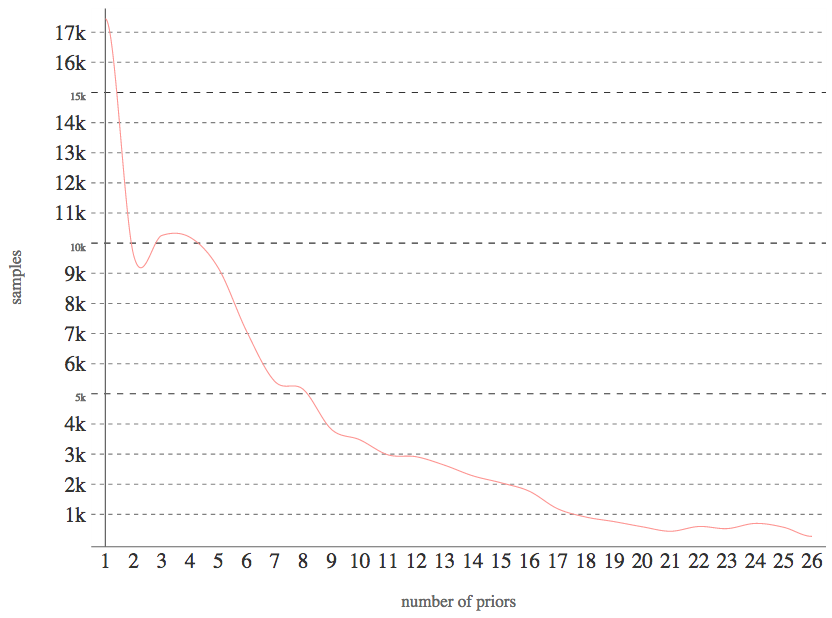
\includegraphics[width=130mm]{chapters/plots/priors_distribution.png}
\caption{Numero di campioni per numero di prior username  \label{overflow}}
\end{figure}

\subsection{Variare le classi di social networks}
Come visto in 3.1.2 esistono 5855 coppie di social networks che contengono almeno una coppia di username, e il numero di situazioni possibili aumenta ora che stiamo considerando di variare il social network di partenza (dello username candidate) e quello degli username priors, che può essere più di uno. Testeremo empiricamente variando e filtrando sia username candidate che username priors per i social networks ritenuti più popolari.

\subsection{Variare il numero di features - Features selection}
Utilizzando tutte le classi e funzioni di features viste nel secondo capitolo si ottiene un vettore di 358 features. Restringeremo le classi di features utilizzate per l'algoritmo di apprendimento analizzando le performance del classificatore al variare di queste. Proveremo in un primo momento a limitare le classi di features applicate empiricamente, per analizzarne i risultati. Eseguiremo in seguito un'approccio di \textit{feature selection}, in particolare utilizzeremo \textit{Principal Component Analysis} o PCA. Lo scopro principale dei due approcci è quello di rimuovere il rumore e aumentare l'efficienza computazionale mantenendo solamente le informazioni “utili” e discriminatorie, per evitare overfitting o il problema noto come \textit{curse of dimensionality}.
Riferendoci alle features descritte nel secondo capitolo, assegnamo un'etichetta ad alcuni sottoinsiemi di queste e mostriamo i risultati ottenuti utilizzando questi insiemi limitati di features:

\begin{itemize}
	\item ALL - Tutte le features
	\item K - DVORAK layout keyboard Exogenous features
	\item Q - QWERTY layout keyboard Exogenous features
	\item X - All Exogenous features (K+Q)
	\item E - Endogenous features
	\item H - Human Limitations features
	\item D - Distances features
\end{itemize}


\section{Modelli di classificazione e risultati}
Per l'implementazione dei modelli di classificazione utilizzati in questo capitolo si fa riferimento alla libreria SciKit Learn\footnote{”scikit-learn - Machine Learning in Python”, http://scikit-learn.org}, un insieme di moduli Python per machine learning e data mining.

In fase di sviluppo, quando ancora non tutte le features erano state realizzate e avevamo un insieme molto limitato del dataset attuale, utilizzavamo Support Vector Machine (SVM) come modello di apprendimento. Le versioni che davano i risultati migliori erano quelle che utilizzavano un kernel RBF. Ad ogni modo, affrontando il problema utilizzando SVM senza kernel, portava a performance simili, indicandoci che probabilmente il problema era risolvibile linearmente. Con il crescere del numero delle features e dei samples a disposizione, crescevano anche i tempi di esecuzione dell'algoritmo e la memoria richiesta dal calcolo, diventando troppo onerosi. È nata così la necessità di passare a un modello di classificatori diversi, conosciuti come “online”, che hanno permesso di affrontare il problema con risorse di tempo e memoria molto più limitate. Non escludiamo che, a fronte di potenza di calcolo e memoria adeguata, SVM avrebbe potuto performare meglio dei modelli di classificazione utilizzati di seguito.

\subsection{Classificatori binari online}

Quello che definisce l'apprendimento online è il modo in cui gli esempi del training set vengono presentati all'algoritmo. Se infatti gli algoritmi di apprendimento fanno in generale l'assunzione di poter vedere il dataset interamente, quelli online hanno la limitazione di poter vedere un esempio alla volta, generalmente applicando questo schema ripetutamente:

\begin{enumerate}
	\item Viene osservata un'istanza
	\item L'algoritmo predice un'etichetta per l'istanza che può essere +1 o -1
	\item Viene rivelata la vera etichetta
	\item L'algoritmo subisce una perdita\footnote{Secondo una funzione di perdita, conosciuta come \textit{loss hinge function}} che riflette il grado di errore della predizione appena eseguita, e aggiorna il suo stato interno.
\end{enumerate}


Questo modo di agire presenta alcuni vantaggi:

\begin{itemize}
	\item Gli algoritmi online possono essere addestrati incrementalmente: se nuovi esempi
si rendono disponibili dopo che il classificatore ha già appreso un modello, questo non deve essere scartato per reiniziare da capo l'apprendimento, ma l'algoritmo aggiorna naturalmente il modello pre-esistente con le nuove informazioni.
	\item Essendo obbligati a vedere il dataset solo un punto alla volta, questi algoritmi sono computazionalmente più efficienti: il dataset può in linea di principio essere disponibile in memoria anche solo un punto alla volta (lasciando il resto sulle periferiche), diminuendo le richieste in spazio.
Queste caratteristiche rendono gli algoritmi online una buona scelta per gestire insiemi di dati di grandi dimensioni.
\end{itemize}


\subsubsection{Stochastic Gradient Descent}
Stochastic Gradient Descent\cite{gardner1984learning} (SGD) è un semplice ma efficiente approccio per modelli discriminativi di classificatori lineari. Anche se SGD è presente da molto tempo nella comunità di machine learning, ha ricevuto solo recentemente una considerabile attenzione nel contesto di apprendimento su larga scala\cite{zhang2004solving}. SGD è stato applicato con successo a problemi di apprendimento automatico con dati sparsi e su grande scala, spesso incontrati in \textit{text classification} e \textit{natural language processing}. Essendo i dati sparsi, il classificatore scala facilmente problemi che presentano anche più di $10^5$ samples e $10^5$ features.\newline
I vantaggi di Stochastic Gradient Descent sono:
\begin{itemize}
	\item Efficienza
	\item Semplicità di implementazione
\end{itemize}
Gli svantaggi di Stochastic Gradient Descent includono:
\begin{itemize}
	\item SGD è sensibile e richiede un certo numero di iperparametri
	\item SGD è estremamente sensibile alla normalizzazione delle features
\end{itemize}

Testiamo ora le performance di questo modello, utilizzando come samples l'intero dataset a disposizione ($\sim$103000 samples). Eseguiremo più test, variando il sottoinsieme di features utilizzate.\newline

\begin{tabular}{ |l|l|l|l|l| }
	\hline
	\textbf{Features} & \textbf{Features length} & \textbf{Accuracy} & \textbf{F1}  & \textbf{AUC} \\ \hline
	ALL & 358 & 93.53\% & 93.22\% & \textbf{93.53\%} \\ \hline
	Q+E+H+D & 274 & 93.49\% & 93.19\% & 93.49\% \\ \hline
	D+Q & 194 & 92.14\% & 91.72\% & 92.14\% \\ \hline
	E+H+D & 190 & 93.45\% & 93.14\% & 93.45\% \\ \hline
	E+D & 182 & 93.27\% & 92.94\% & 93.27\% \\ \hline
	D+H & 18 & 92.08\% & 91.57\% & 92.08\% \\ \hline
	D & 10 & 91.55\% & 91.94\% & 91.54\% \\
	\hline
\end{tabular}
\newline\newline

In grassetto, la configurazione che ottiene i risultati migliori. Si nota che è la configurazione che utilizza tutte le features ad ottenerli, ma si nota anche che al decrementare, anche ingente, di numero di features le performance non scendono altrettanto velocemente.\newline

Testiamo ora le performance, utilizzando come samples filtrando il dataset dei profili con associati un solo priors, usando quindi come minimo due priors username ($\sim$85300 samples). Anche qui, eseguiremo più test, variando il sottoinsieme di features utilizzate.\newline


\begin{tabular}{ |l|l|l|l|l| }
	\hline
	\textbf{Features} & \textbf{Features length} & \textbf{Accuracy} & \textbf{F1}  & \textbf{AUC} \\ \hline
	ALL & 358 & 93.85\% & 93.60\% & 93.84\% \\ \hline
	E+D & 182 & 94.04\% & 93.77\% & \textbf{94.03\%} \\ \hline
	D+H & 18 & 93.16\% & 92.54\% & 93.14\% \\ \hline
	D & 10 & 92.36\% & 91.79\% & 92.34\% \\
	\hline
\end{tabular}
\newline\newline

Notiamo che in generale l'efficienza del classificatore e in particolare l'accuratezza aumentano, con ogni sottoinsieme di features. In questo caso il risultato migliore è peró ottenuto utilizzando un sottoinsieme di features e non l'insieme completo. Notiamo comunque che anche in questo caso, il sottoinsieme limitato di features D, porta a risultati accettabili.\newline

Decidiamo ora di analizzare l'andamento del classificatore filtrando il dataset variando il numero minimo di priors e utilizzando solamente il sottoinsieme di 10 features contenute in D. In Fig 4 riportiamo i dati analizzati, attraverso un grafo che li riassume. Usando un set ristretto di solo 10 features, il classificatore spazia da una accuratezza del 91.5\% utilizzando l'intero dataset fino a una accuratezza del 100\% utilizzando i profili con il massimo numero di priors username (26).


\begin{figure}[bp!]
\centering
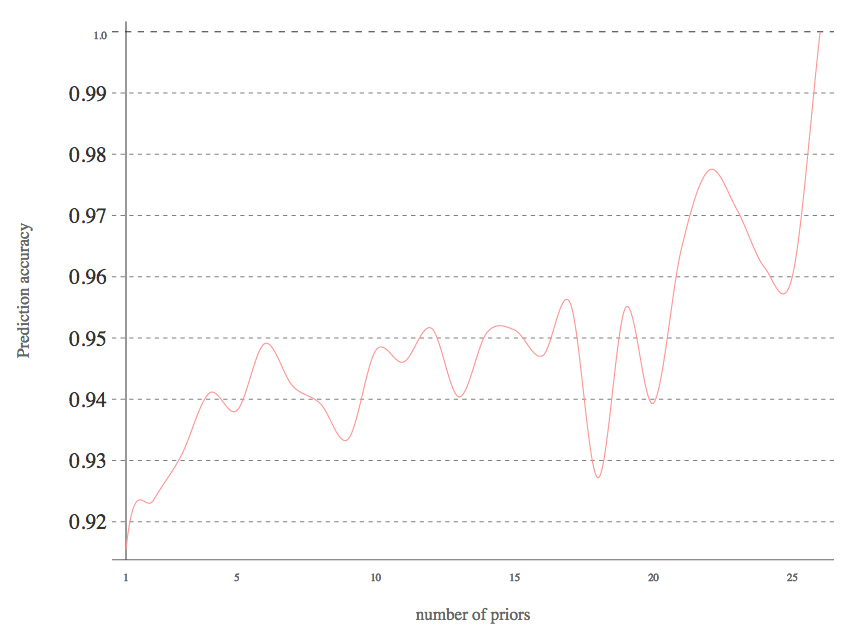
\includegraphics[width=130mm]{chapters/plots/accuracy_distribution.png}
\caption{SGD Accuracy performance con differenti numeri di priors username \label{overflow}}
\end{figure}

\subsubsection{Passive Aggressive}

Passive Aggressive \cite{crammer06}, abbreviato come PA, è un altro algoritmo di apprendimento online. Il suo nome è dovuto al comportamento di reazione alla perdita descritta in 4.3.1.
La funzione di perdita in PA ritorna valore 0 quando il margine di accuratezza della predizione risulta essere almeno unitario. Altrimenti equivale alla differenza tra il valore di margine e 1. Il comportamento di PA, dunque, risulta passivo nel caso in cui la perdita equivalga a 0, ovvero lo stato interno del classificatore non varia e verrà restituito l'iperpiano di partenza. In caso di perdita maggiore di 0, il classificatore reagirà aggressivamente, restituendo ad ogni costo un iperpiano che soddisfi il requisito di margine quantomeno unitario. Bisogna però notare come l’aggressività nell’affrontare questo problema possa essere eccessiva in alcune situazioni reali. Infatti, è comune nella pratica avere nei dati di esempio una certa quantità di rumore sulle etichette (alcune di esse possono essere non corrette dato il vettore di esempio). Uno di questi esempi mal classificati potrebbe causare, se l'algoritmo forzasse l’ottenimento su di esso di un margine 1, la distruzione di un iperpiano che fino a lì aveva dato ottimi risultati. Per correggere ciò, gli autori introducono una versione in cui l’aggressività è calibrata da un parametro C.



Testiamo ora le performance di PA, utilizzando come samples l'intero dataset a disposizione ($\sim$103000 samples). Eseguiremo più test, variando il sottoinsieme di features utilizzate.\newline

\begin{tabular}{ |l|l|l|l|l| }
	\hline
	\textbf{Features} & \textbf{Features length} & \textbf{Accuracy} & \textbf{F1}  & \textbf{AUC} \\ \hline
	ALL & 358 & 91.44\% & 91.22\% & 91.43\% \\ \hline
	D+H & 18 & 91.42\% & 90.77\% & 91.32\% \\ \hline
	D & 10 & 91.66\% & 90.84\% & \textbf{91.64\%} \\
	\hline
\end{tabular}
\newline\newline

Generalmente con questo algoritmo si ottiene una prestazione peggiore che con SGD. Notiamo però che PA sembra essere meno sensibile alla riduzione del numero di features.

\section{Risultati}

Abbiamo testato due algoritmi di classificatori binari online, Stochastic Gradient Descent e Passive Aggressive ottenendo risultati diversi. Stochastic Gradient Descent porta generalmente a risultati migliori, ma risulta più sensibile al variare di numero di features rispetto a PA che invece mantiene un'accuratezza quasi costante al variare di queste.\newline
Riassumendo, riteniamo Stochastic Gradient Descent l'algoritmo migliore per affrontare il problema di categorizzazione preposto in questa tesi, e individuiamo Passive Aggressive come algoritmo con risultati migliori per un numero ristretto di features.\newline
Riporto due tabelle che riassumono i risultati appena descritti, la prima mostra le performance dei due algoritmi ottenuti utilizzando l'intero dataset e l'intero insieme features descritte nel secondo capitolo. La seconda tabella riporta le performance ottenute utilizzando un sotto insieme delle features, classificate con l'etichetta D in 4.2.3. \newline

\begin{tabular}{ |l|l|l| }
	\hline
	\textbf{Model} & \textbf{Accuracy} & \textbf{AUC} \\ \hline
	Stochastic Gradient Descent & 93.53\% & \textbf{93.53\%} \\ \hline
	Passive Aggressive &  91.34\% & 91.36\% \\
	\hline
\end{tabular}
\newline\newline

\begin{tabular}{ |l|l|l| }
	\hline
	\textbf{Model} & \textbf{Accuracy} & \textbf{AUC} \\ \hline
	Stochastic Gradient Descent & 91.55\% & 91.54\% \\ \hline
	Passive Aggressive &  91.66\% & \textbf{91.64\%} \\
	\hline
\end{tabular}
\newline\newline

\section{Comparazione con il lavoro svolto da Zafarani et al}

Presentiamo ora alcune differenze che sussistono tra il lavoro svolto in questa tesi e quello condotto da Zafarani et al. Le differenze si distinguono in:

\begin{enumerate}
	\item Differenze nel dataset
	\item Differenze nelle features implementate
\end{enumerate}


Per quanto riguarda il primo punto, vi sono più aspetti che differiscono. I due dataset differiscono per quantità, fonti, omogeneità dei SNS considerati, predisposizione dei dati ad essere classificati.

Il dataset raccolto da Zafarani et al è stato collezionato da diverse fonti\cite{zafarani13}:
\begin{itemize}
	\item Social Networking Sites as \textit{Facebook} or \textit{Google+} public data
	\item Blog portals as \textit{BlogCatalog}
	\item Forums
\end{itemize}

Da queste fonti hanno collezionato $\sim$100000 coppie (c-U) dove c è uno username e U l'insieme di priors username e sia c che U appartengono allo stesso individuo. Il loro dataset conteneva username da 32 diversi siti. Le istanze negative sono state estratte da quelle positive in maniera simile a quella proposta da noi in 4.1, e bilanciate con il numero di istanze positive, raggiungendo $\sim$200000 istanze. Menzioniamo il fatto che il dataset raccolto nel lavoro di Zafarani risulta essere predisposto alla classificazione per le seguenti motivazioni. Su questo dataset, un sistema naive di classificazione ottiene il 77\% di accuratezza. Questo sistema viene indicato nel lavoro di Zafarani come “Exact username Match, a baseline method for comparison” e opera come descritto qui sotto.
\paragraph{\textit{em}: ‘Exact username Match - baseline method for comparison’}
Considera un istanza positiva se lo username candidato corrisponde esattamente(“\textit{exact match}”) per il $\alpha$\% degli username. Per impostare $\alpha$ accuratamente, si computa la percentuale di prior username che corrisponde esattamente al candidate username per ognuna delle istanze positive del dataset e ne viene calcolata la media secondo tutte le istanze positive.\newline\newline
Per il dataset di Zafarani, $\alpha$ viene riportato con un valore di $\sim$54\%. Per meglio analizzarne l'impatto, riportano, impostano 50\% $\leq$ $\alpha$ $\leq$ 100\%.
Nel migliore dei casi, con $\alpha$ = 50\%, il classificatore raggiungerebbe un'accuratezza del 77\%.\newline
Sul nostro dataset, \textit{em} con $\alpha$ = 50\%, avrebbe un accuratezza del 59\%.
Nel nostro caso comunque, $\alpha$ pesato, calcolato come descritto precedentemente, assume un valore di $\sim$ 21\%. Con questo valore, \textit{em} sul nostro dataset raggiunge un'accuratezza del $\sim$ 67\%. Inoltre, il dataset di Zafarani, presenta un maggior numero di profili. Riassumo le differenze dei due dataset in una tabella.\newline




\begin{tabular}{ |l|l|l|l|l|l| }
	\hline
	 & \textbf{samples} & \textbf{different SNS} & \textbf{$\alpha$} & \textbf{\textit{em}} & \textbf{\textit{em} $\alpha$ = 50\%} \\ \hline
	Zafarani et al & $\sim$200000  & 32 & $\sim$54\%  & \textless 77\%  & 77\%\\ \hline
	Questa tesi &  $\sim$100000 & 168 & $\sim$21\%  & 67\%  & 59\% \\
	\hline
\end{tabular}
\newline\newline

Una seconda discrepanza con il lavoro di Zafarani si può osservare nel numero di features implementato. Non tutte le features presentate\cite{zafarani13} sono state infatti implementate. Altre invece, sono state aggiunte e proposte da noi. In somma, l'insieme completo delle features proposte da Zafarani conta 414 features, quelle proposte in questa tesi 358. In particolare, in questa tesi abbiamo testato le performance del classificatore utilizzando un insieme ristretto di features (10), che corrisponde a quelle introdotte da noi e che non compaiono tra quelle implementate da Zafarani. Queste sono le features etichettate come “di distanza” nel capitolo 2 e indicate con l'etichetta “D” in 4.2.3.

Ad ogni modo, anche Zafarani ha condotto un test limitando a 10 il numero di features, utilizzando \textit{odd-rations} o OR, una misurazione che descrive la forza di associazione o dipendenza tra due valori binari, che ricopre un ruolo importante nella regressione logistica, modello utilizzato da Zafarani per affrontare il problema di classificazione.

L'idea di usare il set limitato di features “D” invece, ci viene suggerito dall'analisi della distribuzione della similarità degli username condotta in 3.1.3, dove si è notato che le classi positive e le classi negative mostravano un pattern visibilmente diverso.\newline

\begin{tabular}{ |l|l|l|l|l| }
	\hline
	& \textbf{technique} & \textbf{features} & \textbf{AUC} & \textbf{Accuracy} \\ \hline
	Zafarani et al & Logistic Regression & ALL(414) & 0.95 & 93.80\% \\ \hline
	Questa tesi &  SGD & ALL(358) & 0.93 & 93.53\% \\ \hline
	Zafarani et al & Logistic Regression & 10 & N/A & 92.72\% \\ \hline
	Questa tesi & Passive Aggressive & 10 & 91.46\% & 91.64\% \\
	\hline
\end{tabular}
\newline\newline
